\chapter{Entwurfsmuster}
\section{Entwurfsmuster: Erbauer}
Die Erzeugung eines Match-Objektes wurde mit Hilfe eines Erbauers realisiert.
Dies ermöglichte eine erhöhte Lesbarkeit und Verständlichkeit: Durch den Einsatz des Builder-Musters wurde der Code lesbarer und einfacher zu verstehen, insbesondere da die Match-Klasse viele Parameter erwartet.
Der Einsatz ermöglichte zudem mehr Flexibilität. Bei Verwendung des Konstruktors hätten entweder separate Konstruktoren für verschiedene Kombinationen von Parametern bereitstellen oder Parameter auf einen Standardwert gesetzt werden müssen, wenn sie nicht angegeben worden wären.
Zuletzt ermöglichte der Einsatz des Erbauers eine Trennung von Erstellungslogik und Geschäftslogik. Das Builder-Muster ermöglicht es, die Erstellungslogik des eher komplexen Match-Objekts von seiner Geschäftslogik zu trennen. Das macht den Code übersichtlicher und einfacher zu warten und zu erweitern.\newpage
\begin{figure}[ht]
    \centering
    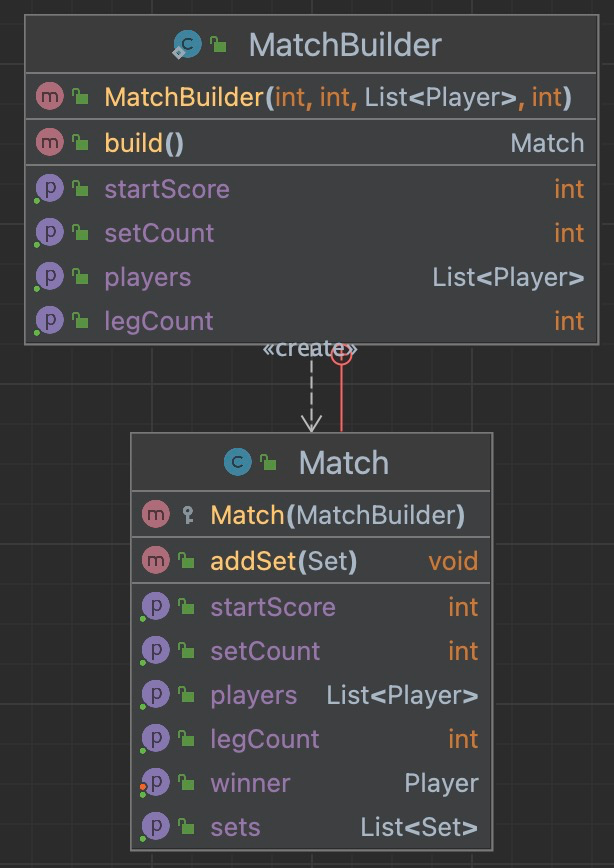
\includegraphics[width=0.5\textwidth]{Bilder/MatchBuilder.png}
    \caption{MatchBuilder}
    \label{fig:matchbuilder}
\end{figure}
\lstinputlisting[
	label=code:match-klasse,    % Label; genutzt für Referenzen auf dieses Code-Beispiel
	caption=Match-Klasse,
	captionpos=b,               % Position, an der die Caption angezeigt wird t(op) oder b(ottom)
	style=EigenerJavaStyle,     % Eigener Style der vor dem Dokument festgelegt wurde
	firstline=1
]{Quellcode/Match.java}
\section{Entwurfsmuster: Strategie}
Das Strategie-Entwurfsmuster bietet erhebliche Flexibilität, da es ermöglicht, das Verhalten von Objekten zur Laufzeit dynamisch zu ändern. Es fördert die Wiederverwendbarkeit und Austauschbarkeit von Algorithmen und erleichtert die Entkopplung von spezifischen Verhaltensweisen von den Klassen, die verwendet werden. Dadurch wird der Code sauberer und einfacher zu warten.\\
\lstinputlisting[
	label=code:handle,    % Label; genutzt für Referenzen auf dieses Code-Beispiel
	caption=Handle-Klasse,
	captionpos=b,               % Position, an der die Caption angezeigt wird t(op) oder b(ottom)
	style=EigenerJavaStyle,     % Eigener Style der vor dem Dokument festgelegt wurde
	firstline=1
]{Quellcode/Handle.java}
Umgesetzt wurde das Entwurfsmuster mit Hilfe der Handle-Klasse, die den Handle-Klassen eine Methode \textit{process} bereitstellt, die den jeweiligen Teil des Dartspiels durchlaufen lassen. Dieses Interface wird dann von allen Handle-Klassen implementiert.\\
\begin{figure}[ht]
    \centering
    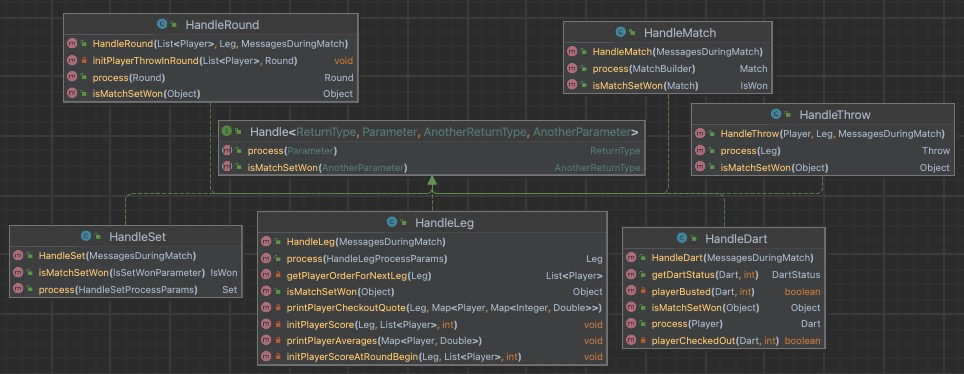
\includegraphics[width=1\textwidth]{Bilder/handleuml.png}
    \caption{Implementierung der Handle Klasse im UML}
    \label{fig:handleuml}
\end{figure}